\chapter{Discussion}
\label{ch:discussion}

Talk about how in hindsight ca and sa weren't the best choices: strips of land on ca are quite thin so may be dominated by coastal effects and has confounding orography, while the extents for sa may be too large and the arc of deforestation is a creeping boundary.

Talk about how WA results may not be generalisable to others due to dry/arid environment.

\begin{figure}[!ht]
	\centering
	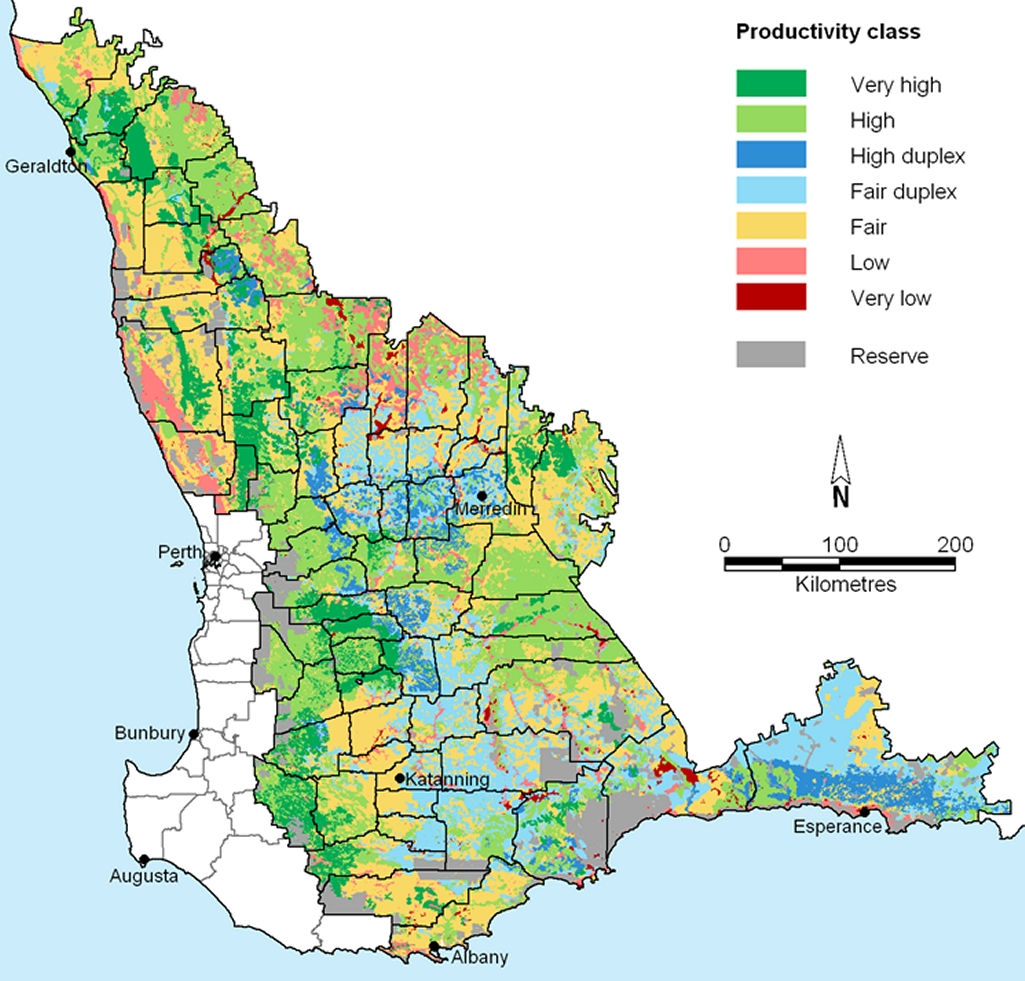
\includegraphics[width=0.9\textwidth]{lc_wa}
	\caption[Western Australia Land Usage]{The Wheat Belt of Western Australia, with shading indicating level of productivity \citep{dpird_2021}.}
	\label{fig:lc_wa}
\end{figure}

\begin{figure}[!ht]
	\centering
	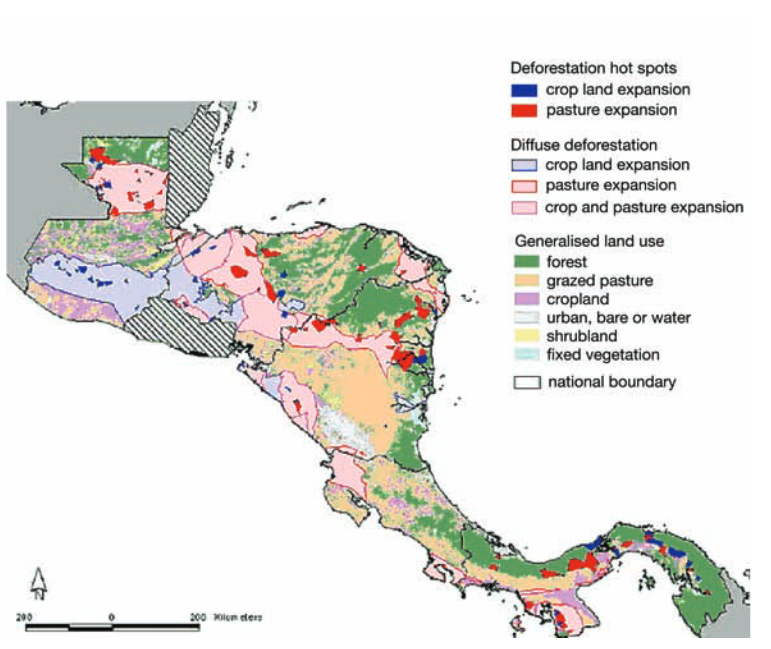
\includegraphics[width=0.9\textwidth]{lc_ca}
	\caption[Central America Land Usage]{Land usage and land cover change in Central America \citep{ipcc_2007}.}
	\label{fig:lc_ca}
\end{figure}

\begin{figure}[!ht]
	\centering
	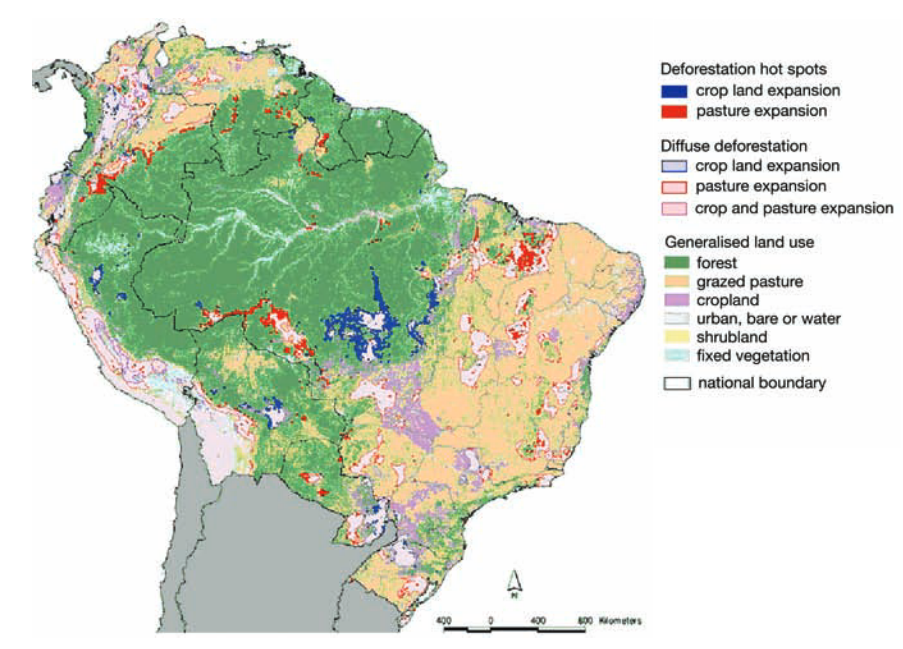
\includegraphics[width=0.9\textwidth]{lc_sa}
	\caption[Northern Brazil Land Usage]{Land usage and land cover change in Northern South America \citep{ipcc_2007}.}
	\label{fig:lc_sa}
\end{figure}

\section{Interpretation of results}

\section{Comparison with literature}

\section{Conceptual framework for local circulations}

We present here a conceptual framework for local circulations based on heuristical principles. We do not suggest that the following is a rigorous formulation but we do believe it captures the general features while being internally consistent, and explains much of the seemingly disparate findings noted in the literature (see Section~\ref{ssec:model_explain}): urban-induced convective storms over the Sydney basin \citep{gero2006}, increased cloud cover and rainfall over small deforested areas in the Amazon but the opposite for large deforested areas \citep{khanna2017}, increasing rainfall with increasing amount of deforestation with no apparent trend reversal in coastal Southern West Africa \citep{taylor2022}, clouds forming first and bunching up on the native vegetation of the fence in Western Australia \citep{lyons2002}, preferential cloud formation in Western Australia over agricultural land in Winter but native vegetation in Summer \citep{ray2003}, increases of precipitation towards forest edges but decreases away from edges in Southwestern Amazonia \citep{knox2011}, increased rainfall downwind of deforested areas \citep{khanna2017}, concentration of convective cores during the evening transition window in coastal Southern West Africa \citep{taylor2022}, and contrasting effects of small-scale deforestation on cloud cover for different forest types \citep{xu2022}.

\subsection{Main circulation drivers from first principles}

\begin{itemize}
	\item All wind energy ultimately derives from solar energy and can be divided into: internal (thermal) energy, latent energy, kinetic energy and gravitational potential energy.
	\item Initiation or strengthening of a convective circulation corresponds to an increase in kinetic energy (local to the volume of air in circulation), and as the sun does not directly impart kinetic energy upon the air, energy for this must be derived from internal, latent or gravitational potential energy (which the sun’s energy first induces changes upon).
	\item Gravity by itself cannot be a driver for convective circulations because it is always directed downward. To be clear, gravity does play a mediating role as conversions from internal and latent energy into kinetic energy often undergoes an intermediate energy conversion into gravitational potential energy first. The downwards direction of gravity imparts a directional preference for circulations upon internal energy conversion into kinetic (colder air masses sink while warmer air masses rise due to their relative densities), and as we’ll argue later, also for latent energy conversion into kinetic.
	\item In an idealised circulation which is localised in space, the long-run average conversion of gravitational potential energy to kinetic is zero as parcels of air that go up also come down in the other leg of the circulation. This is in contrast to internal and latent energy conversion into kinetic which may derive from external inputs into the local circulation (via radiative heating and moisture transport respectively). It is in this sense that we mean that gravity cannot drive circulations.
	\item Thus the main drivers for convective circulations must be:
	\begin{itemize}
		\item Temperature gradients (associated mostly with diurnal heating patterns and energy balance for different surfaces): internal energy is lost as heated air decompresses to equalise built up pressure from surface heating and cools down in the process of doing so (under approximate assumptions of ideal gas so that PV = nRT and that the total volume of air in circulation is changing relatively slowly).
		\item Atmospheric condensation (i.e.\ cloud formation): latent energy stored in water vapour is lost as the accumulated moisture from evapotranspiration condenses out and is used up by clouds.
		\item In both of the above processes, energy is conserved since heated air (whether from built up internal energy or latent heat warming) eventually cools down in the return circulation so that average kinetic power generation within the volume of air in circulation is approximately zero \textit{in the absence of external energy input into the system}. However, the sun \textit{does} contribute an input of energy into the system in the form of daytime heating producing internal (thermal) energy and evapotranspiration of liquid water producing latent energy.
		\item A crucial distinction is that whereas the former contribution is mostly localised in space and time to the volume and event of the circulation, the latter contribution is not necessarily so. Latent energy buildup can occur at a distant point in space and over a relatively long period, then at a later time enter the volume of air in circulation. The implications of this are discussed later.
		\item The condensation-induced airflows will be anisotropic and directed upwards. The possibility for anisotropic airflow is convincingly demonstrated in a series of experiments by \citet{bunyard2015, bunyard2017, bunyard2019}. See Appendix~\ref{sec:anis_cond} for a heuristical argument as to the causes of this anisotropy.
	\end{itemize}
\end{itemize}

\subsection{The effect of temperature gradients}

\begin{itemize}
	\item Areas with higher temperatures are associated with lower surface pressure (as air rises).
	\item Areas with lower temperatures are associated with higher surface pressure (as air sinks).
	\item Temperature at each surface is in turn governed by the surface energy balance $SLHF + SSHF = R_n - G$ where $R_n$ is net radiation and $G$ is ground flux.
	\item $R_n$ is determined mostly by albedo, surface thermal properties and solar irradiance (which may be affected by cloud cover).
	\item $G$ is determined mostly by soil moisture (for vegetation cover) and surface thermal properties (for urban cover), and for vegetation cover can in many cases be assumed approximately proportional to $R_n$ \citep{lyons1996}.
	\item The partitioning between \ac{SLHF} and \ac{SSHF} is determined primarily by plant species behaviour in relation to environmental factors such as soil moisture, temperature, solar irradiance, etc. for natural and agricultural land cover. For agricultural lands, these factors fluctuate significantly according to the cropping cycle and as a result so too does this energy partitioning.
	\item The greater the evapotranspiration the greater the \ac{SLHF}, and so for the same $R_n$ (assuming $G$ is proportional to $R_n$) this means lower \ac{SSHF}.
	\item \ac{SSHF} in turn ends up being
	\begin{itemize}
		\item The thermal energy of the surface air mass as air heats up via conduction with the surface: an account of this can be used to assess likely temperature gradients.
		\item The kinetic energy and gravitational potential energy from local scale convections and turbulent mixing with the result that air parcels reach a greater height and hence \ac{BLH} is increased.
	\end{itemize}
	\item \ac{SLHF} corresponds with the amount of moisture being added into the atmosphere in the form of water vapour, which in turn increases relative humidity and hence a decrease in \ac{LCL}.
\end{itemize}

\subsection{The effect of atmospheric condensation}

\begin{itemize}
	\item Atmospheric condensation occurs when \ac{BLH} is greater than \ac{LCL} and there is sufficient atmospheric moisture.
	\item Sustained condensation requires a continued supply of atmospheric moisture.
	\item A low pressure region forms under and around the area of condensation, which induces a circulation (whereby air is directed upward towards the site of condensation, then outward and downward in a return circulation).
	\item Shortly after initiation of condensation, a horizontal pressure gradient forms (due to the sudden loss in volume from water vapour condensing to liquid form) which advects surrounding moisture to sustain continued condensation. The upward air motion immediately preceding this and which was then directed outward eventually replaces the advected air to conserve matter fluxes. Meanwhile, to conserve energy fluxes, the latent heat released above cloud base and which was contained by air in the return leg of the circulation is eventually absorbed by surface air (which would have lost heat in the process of decompressing in the presence of the horizontal pressure gradient).
\end{itemize}

\subsection{Heuristical procedure for qualitatively assessing likely effect of land cover on strength and direction of circulations}

\begin{enumerate}
	\item Assess the \ac{BLH} at each point in the study region.
	\begin{itemize}
		\item For calm conditions, this is determined primarily by (and positively correlated with) the \ac{SSHF} at each point.
		\item For windy conditions, this is determined by
		\begin{itemize}
			\item The \ac{SSHF} \textit{upwind} of each point (since wind traversing through the upwind region is subjected to buoyancy forces determined by the \ac{SSHF} in that upwind region, and is then carried through by its inertia, arriving at an increased height by the time it reaches each point.
			\item The surface roughness (the rougher the surface the more turbulent mixing and so the higher the \ac{BLH})
			\item \textit{Upwind} orography (as winds may be deflected upwards upon hitting an incline)
		\end{itemize}
		\item Apart from upwind orography, localised peaks in the \ac{BLH} at each point may also occur where there is an abrupt interface \textit{upwind} where winds go from a surface with lower to higher roughness (in a similar effect to that of orography, the winds are slowed down and concentrate near the interface then must extend vertically to equalise the pressure buildup). This is unless the region of lower roughness happens to be very short along the direction of wind travel, and there exists another surface immediately upwind with a roughness equal to or higher than the downwind high roughness surface (because this implies a lower volume of space for the winds to expand into then deflect upwards from upon reaching the second interface).
		\end{itemize}
	\item Assess the \ac{LCL} at each point in the study region.
	\begin{itemize}
		\item This is a function of surface temperature, pressure and \ac{RH}, but mostly \ac{RH}.
		\item For initially calm conditions, \ac{RH} is determined primarily by evapotranspiration, for which \ac{SLHF} is an indicator for. \ac{RH} for areas without high evapotranspiration but with a characteristic spatial scale much smaller than neighbouring areas which have high evapotranspiration may also have high humidity as neighbouring moisture drifts towards it.
		\item For windy conditions, \ac{RH} is determined primarily by \textit{upwind} evapotranspiration, for which \ac{SLHF} is a proxy for. However, unlike the case for \ac{SSHF} with regards to \ac{BLH} where the \ac{BLH} at each point is determined by \ac{SSHF} immediately upwind of the point, the evapotranspiration / \ac{SLHF} can be of a very remote origin if there is negligible upwind condensation (i.e.\ winds may carry moisture from afar as in the case of a sea breeze).
	\end{itemize}
	\item Identify areas where \ac{BLH} is greater than \ac{LCL}.
	\begin{itemize}
		\item These are areas where atmospheric condensation (cloud formation) will occur.
		\item The atmospheric condensation will induce a local decrease in surface pressure and advect moisture towards itself (at least on local scales, and possibly larger scales).
	\end{itemize}
	\item Assess for these areas what the following moisture flow is likely to be, in context of the synoptic background.
	\begin{itemize}
		\item If there is sufficient moisture local to where the atmospheric condensation is occurring, or there is sufficient moisture from far away sources (e.g.\ a sea breeze, in which case \ac{SST} needs to be considered) which synoptic conditions are not inhibiting, then the atmospheric condensation can be sustained and a circulation will develop such that surface winds (and moisture) are directed towards the sites of atmospheric condensation (at least on local scales). The greater the amount of condensation, the more intense the circulation and winds.
		\item As regards circulations and winds at a larger (e.g.\ synoptic) scale, the Coriolis force needs to be taken into consideration when the study region is outside of the Tropics.
		\item Sustained atmospheric condensation may also inhibit nearby cloud formation due to advection of moisture from neighbouring regions but also because the downward leg of the resulting circulation may increase the surface pressure of neighbouring regions (i.e.\ downward winds prevent moist air from rising to the \ac{LCL}). This in turn may increase the net radiation and hence evapotranspiration from nearby vegetation, providing even more moisture to sustain continued atmospheric condensation (and hence the circulation).
		\item As such, subsequent circulation and convective developments may be dependent on initial conditions as to where and with what spatial pattern the atmospheric condensation first manifests.
	\end{itemize}
	\item Assess the temperature gradient across different surfaces.
	\begin{itemize}
		\item All other things equal, circulations should be such that surface winds move from cooler regions (higher surface pressure) to warmer regions (lower surface pressure).
		\item If \ac{BLH} is less than \ac{LCL} at almost all points or there is insufficient moisture for sustained atmospheric condensation at the points where \ac{BLH} is greater than \ac{LCL}, then the temperature gradient effect should dominate.
		\item For cases where the predicted wind flow from atmospheric condensation and temperature gradients oppose each other, the relative contribution of each mechanism needs to be considered.
	\end{itemize}
	\item Some rules of thumb in assessing \ac{SSHF} and \ac{SLHF}.
	\begin{itemize}
		\item Agricultural land cover typically employ annual crops, which compared with natural land cover have higher albedo (lower \ac{SSHF} + \ac{SLHF} total), lower roughness, and greater annual variation in the Bowen ratio (which is lower during the growing season). Where there is bare land cover after harvest which persists until the next growing season, the albedo and Bowen ratio is likely to be especially high. Where there is dry soil, clearing of vegetation may actually increase \ac{SSHF} despite increases in albedo, as the Bowen ratio increases.
		\item Natural land cover such as native vegetation and forests, as compared with agricultural land cover, typically have lower albedo (higher \ac{SSHF} + \ac{SLHF} total), higher roughness, and a Bowen ratio which is low for ecosystems adapted towards moist conditions but high for dryland species. There will be significantly less annual variation in all 3 of these as compared with agricultural land. Natural land cover will typically have higher \ac{SSHF} than agricultural land unless the latter is so bare that \ac{SLHF} becomes negligible (as can be the case between harvest and the next growing season), while at the same time the former is an ecosystem adapted to wet environments with very low Bowen ratio. 
		\item Differences in \ac{SSHF} and \ac{SLHF} across different land cover types can in part be offset by differences in fractional vegetation cover \citep{mahmood2011}.
		\item Open bodies of water have very low Bowen ratio and cool surface temperatures so they usually mark the downward leg of a circulation and daytime atmospheric condensation in these areas \textit{may} be suppressed \citep{cutrim1995}.
		\item Urban areas have an albedo which depends on local urban design, but a roughness and Bowen ratio which is typcally higher than both natural and agricultural land cover, and these variables display little annual variation.
	\end{itemize}
\end{enumerate}

\subsection{Speculations}

\begin{itemize}
	\item The initial spatial pattern of atmospheric condensation may affect how much total moisture will be advected to sustain that initial condensation over the course of the circulation’s lifetime. If the same amount of water vapour is condensed over a larger volume of air and over a similar period of time, there is a lower volumetric power density (and weaker pressure gradient force per unit area perpendicular to the base surface of the cloud averaged over the period of condensation) which may not reach a critical threshold for sustained convection. Self-sustaining cumulus formation (and convective memory) is achieved where moisture is being advected into the cloud at a quick enough rate that the resulting local power density will in turn advect more moisture at a quick enough rate to do the same and continue the cycle. In the case that the moisture is oceanic in origin, this may translate to an increase in the average amount of atmospheric condensation and precipitation for each occurrence of a condensation-induced circulation. Even if on average the total atmospheric condensation is independent of initial spatial pattern of formation, the higher volumetric power density associated with condensation over a smaller volume of air may still lead to appreciable effects in circulation such as an increased prevalence of short but intensive bursts (in favour of slow and sustained circulation).
	\item If the above is correct, then biogenic aerosol release (or \ac{SOA} formation from biogenic \ac{VOC}s) may play a role in determining that initial spatial pattern, where subsequent condensation and rainfall will be concentrated, and may also determine the amount of condensation that will occur before the cumulus can no longer sustain its own moisture and the circulation’s lifecycle ends.
	\item If the above 2 speculations are correct, we further speculate that cloud inhibition upon neighbouring areas is a \textit{competitive} mechanism between ecological communities (at least in flat terrain). While the downward leg of the cumulus convection inhibits upwards air movement from neighbouring region, the horizontal return leg also advects away neighbouring moisture and possibly \ac{CCN}. The ability for an ecological community to induce favourable rainfall upon itself constitutes a selectional advantage and the ordered structures required to enforce such a mechanism would be subject to decay over time (e.g.\ due to mutations in individual species, or weeds crowding out and changing the species in an ecological community). The fact that water is essential for terrestrial life and that this mechanism persists to this day suggests that there must have been competitive selection between ecological communities to maintain these ordered structures (whereby communities unable to do so are at a competitive disadvantage and the communities able to do so give rise to progeny who retain this feature) \citep{gorshkov2000}. If this is correct, then in assessing circulation changes due to \ac{LCC}, a distinction needs to be made between natural and managed forests, where ecosystems which have been subjected to greater anthropogenic change are likely to display more chaotic and random initiations in atmospheric condensation.
\end{itemize}

\subsection{Results and literature anomalies cast within conceptual framework}
\label{ssec:model_explain}

\section{Significance}

\section{Limitations and possible improvements}

The study periods are then chosen based on when there has been the greatest change in Leaf Area Index (as measured by the 5-year rolling average of annual difference), as well as the values for relevant multidecadal atmospheric oscillation indices over each period. Regarding the latter, periods which are to be compared with each other are chosen such that the average of the multidecadal atmospheric oscillation indices over each period are similar. These include indices for the Pacific Decadal Oscillation (PDO) and Atlantic Multidecadal Oscillation (AMO). This is a best attempt at controlling for atmospheric oscillations but is not ideal since there are non-linearities associated with these indices (i.e.\ even if if the average is similar, the effects might not be, especially if the time spent in the extremes of the indices for each period are different). There may also be memory effects persisting from recent atmospheric conditions immediately preceding each period.

\section{Future directions for research}

- For the third comparison, we selected a set of periods for which the 5-year averages of relevant climate indicies had \textit{dissimilar} values, hereby referred to a the "dissimilar comparison". The rationale behind this was that were some relationship to be identified in the analysis between \textit{similar} periods, we could evaluate our confidence in that relationship by seeing whether it holds even under extreme differences in atmospheric conditions.

In an ideal world, you should have two kind of evaluations. The first is against some ground truth (perhaps a random model?). The second kind of evaluation is against other people's work (accuracy, speed, etc.). Any dimension which is of interest, should be evaluated.  Evaluation should be statistically sound.

\Blindtext

\section*{Summary}
\blindtext